\documentclass{article}
\usepackage{fancyhdr}
\usepackage{extramarks}
\usepackage{amsmath}
\usepackage{amsthm}
\usepackage{amsfonts}
\usepackage{tikz}
\usepackage[plain]{algorithm}
\usepackage{algpseudocode}
\usepackage{listings} 
\usepackage{neuralnetwork}
\usepackage{subfigure}
\usepackage{xltxtra,fontspec,xunicode}
\usepackage[slantfont,boldfont]{xeCJK} % 允许斜体和粗体
\usepackage{xeCJK}
\setCJKmainfont{PingFangSC-Regular}   % 设置缺省中文字体
\setCJKmonofont{Hei}   % 设置等宽字体
% \setmainfont{Optima}   % 英文衬线字体
\setmonofont{FiraCode-Regular}   % 英文等宽字体
% \setsansfont{Trebuchet MS} % 英文无衬线字体
\usetikzlibrary{automata,positioning}

\usepackage{color}
\definecolor{dkgreen}{rgb}{0,0.6,0}
\definecolor{gray}{rgb}{0.5,0.5,0.5}
\definecolor{mauve}{rgb}{0.58,0,0.82}

\lstset{frame=tb,
  language=Python,
  aboveskip=3mm,
  belowskip=3mm,
  showstringspaces=false,
  columns=flexible,
  basicstyle={\small\ttfamily},
  numbers=none,
  numberstyle=\tiny\color{gray},
  keywordstyle=\color{blue},
  commentstyle=\color{dkgreen},
  stringstyle=\color{mauve},
  breaklines=true,
  breakatwhitespace=true,
  tabsize=3
}
%
% Basic Document Settings
%

\topmargin=-0.45in
\evensidemargin=0in
\oddsidemargin=0in
\textwidth=6.5in
\textheight=9.0in
\headsep=0.25in

\linespread{1.1}

\pagestyle{fancy}
\lhead{\hmwkAuthorName}
\chead{\hmwkClass\: \hmwkTitle}
\rhead{\firstxmark}
\lfoot{\lastxmark}
\cfoot{\thepage}

\renewcommand\headrulewidth{0.4pt}
\renewcommand\footrulewidth{0.4pt}

\setlength\parindent{0pt}

%
% Create Problem Sections
%

\newcommand{\enterProblemHeader}[1]{
    \nobreak\extramarks{}{Task \arabic{#1} continued on next page\ldots}\nobreak{}
    \nobreak\extramarks{Task \arabic{#1} (continued)}{Problem \arabic{#1} continued on next page\ldots}\nobreak{}
}

\newcommand{\exitProblemHeader}[1]{
    \nobreak\extramarks{Task \arabic{#1} (continued)}{Problem \arabic{#1} continued on next page\ldots}\nobreak{}
    \stepcounter{#1}
    \nobreak\extramarks{Task \arabic{#1}}{}\nobreak{}
}

\setcounter{secnumdepth}{0}
\newcounter{partCounter}
\newcounter{homeworkProblemCounter}
\setcounter{homeworkProblemCounter}{1}
\nobreak\extramarks{Task \arabic{homeworkProblemCounter}}{}\nobreak{}

%
% Homework Problem Environment
%
% This environment takes an optional argument. When given, it will adjust the
% problem counter. This is useful for when the problems given for your
% assignment aren't sequential. See the last 3 problems of this template for an
% example.
%
\newenvironment{homeworkProblem}[1][-1]{
    \ifnum#1>0
        \setcounter{homeworkProblemCounter}{#1}
    \fi
    \section{Task \arabic{homeworkProblemCounter}}
    \setcounter{partCounter}{1}
    \enterProblemHeader{homeworkProblemCounter}
}{
    \exitProblemHeader{homeworkProblemCounter}
}

%
% Homework Details
%   - Title
%   - Due date
%   - Class
%   - Section/Time
%   - Instructor
%   - Author
%

\newcommand{\hmwkTitle}{Lab\ \#6}
\newcommand{\hmwkDueDate}{September 25, 2019}
\newcommand{\hmwkClass}{CSCI964 Computational Intelligence}
\newcommand{\hmwkClassTime}{3.5}
\newcommand{\hmwkClassInstructor}{Zhifeng Wang}
\newcommand{\hmwkAuthorName}{\textbf{Mei Wangzhihui}}
\newcommand{\hmwkAuthorNum}{\textbf{2019124044}}
%
% Title Page
%

\title{
    \vspace{2in}
    \textmd{\textbf{\hmwkClass:\ \hmwkTitle}}\\
    % \normalsize\vspace{0.1in}\small{Due\ on\ \hmwkDueDate\ at 3:10pm}\\
    % \vspace{0.1in}\large{\textit{\hmwkClassInstructor\ \hmwkClassTime}}
    \vspace{3in}
}

\author{\hmwkAuthorName\ \hmwkAuthorNum}
\date{}

\renewcommand{\part}[1]{\textbf{\large Part \Alph{partCounter}}\stepcounter{partCounter}\\}

%
% Various Helper Commands
%

% Useful for algorithms
\newcommand{\alg}[1]{\textsc{\bfseries \footnotesize #1}}

% For derivatives
\newcommand{\deriv}[1]{\frac{\mathrm{d}}{\mathrm{d}x} (#1)}

% For partial derivatives
\newcommand{\pderiv}[2]{\frac{\partial}{\partial #1} (#2)}

% Integral dx
\newcommand{\dx}{\mathrm{d}x}

% Alias for the Solution section header
\newcommand{\solution}{\textbf{\large Solution}}

% Probability commands: Expectation, Variance, Covariance, Bias
\newcommand{\E}{\mathrm{E}}
\newcommand{\Var}{\mathrm{Var}}
\newcommand{\Cov}{\mathrm{Cov}}
\newcommand{\Bias}{\mathrm{Bias}}

\begin{document}

\maketitle

\pagebreak

\begin{homeworkProblem}
\begin{lstlisting}


def euler_distance(point1: np.ndarray, point2: list) -> float:
    """
    计算两点之间的欧拉距离,支持多维
    """
    distance = 0.0
    for a, b in zip(point1, point2):
        distance += math.pow(a - b, 2)
    return math.sqrt(distance)


class ClusterNode(object):
    def __init__(self, vec, left=None, right=None, distance=-1, id=None, count=1):
        """
        :param vec: 保存两个数据聚类后形成新的中心
        :param left: 左节点
        :param right:  右节点
        :param distance: 两个节点的距离
        :param id: 用来标记哪些节点是计算过的
        :param count: 这个节点的叶子节点个数
        """
        self.vec = vec
        self.left = left
        self.right = right
        self.distance = distance
        self.id = id
        self.count = count


class Hierarchical(object):
    def __init__(self, k=1):
        assert k > 0
        self.k = k
        self.labels = None

    def fit(self, x):
        nodes = [ClusterNode(vec=v, id=i) for i, v in enumerate(x)]
        distances = {}
        point_num, future_num = np.shape(x)  # 特征的维度
        self.labels = [-1] * point_num
        currentclustid = -1
        while len(nodes) > self.k:
            min_dist = math.inf
            nodes_len = len(nodes)
            closest_part = None  # 表示最相似的两个聚类
            for i in range(nodes_len - 1):
                for j in range(i + 1, nodes_len):
                    # 为了不重复计算距离,保存在字典内
                    d_key = (nodes[i].id, nodes[j].id)
                    if d_key not in distances:
                        distances[d_key] = euler_distance(nodes[i].vec, nodes[j].vec)
                    d = distances[d_key]
                    if d < min_dist:
                        min_dist = d
                        closest_part = (i, j)
                        # 合并两个聚类
            part1, part2 = closest_part
            node1, node2 = nodes[part1], nodes[part2]
            new_vec = [(node1.vec[i] * node1.count + node2.vec[i] * node2.count) / (node1.count + node2.count) for i in range(future_num)]
            new_node = ClusterNode(vec=new_vec, left=node1, right=node2, distance=min_dist, id=currentclustid, count=node1.count + node2.count)
            currentclustid -= 1
            del nodes[part2], nodes[part1]  # 一定要先del索引较大的
            nodes.append(new_node)
        self.nodes = nodes
        self.calc_label()

    def calc_label(self):
        """
        调取聚类的结果
        """
        for i, node in enumerate(self.nodes):
            # 将节点的所有叶子节点都分类
            self.leaf_traversal(node, i)

    def leaf_traversal(self, node: ClusterNode, label):
        """
        递归遍历叶子节点
        """
        if node.left == None and node.right == None:
            self.labels[node.id] = label
        if node.left:
            self.leaf_traversal(node.left, label)
        if node.right:
            self.leaf_traversal(node.right, label)


def setData(filename):
    #生成num个随机数据
    Data = np.loadtxt(filename, delimiter=',', usecols=(0, 1, 2, 3))
    return Data
\end{lstlisting}
\begin{figure}[]
    \centering
    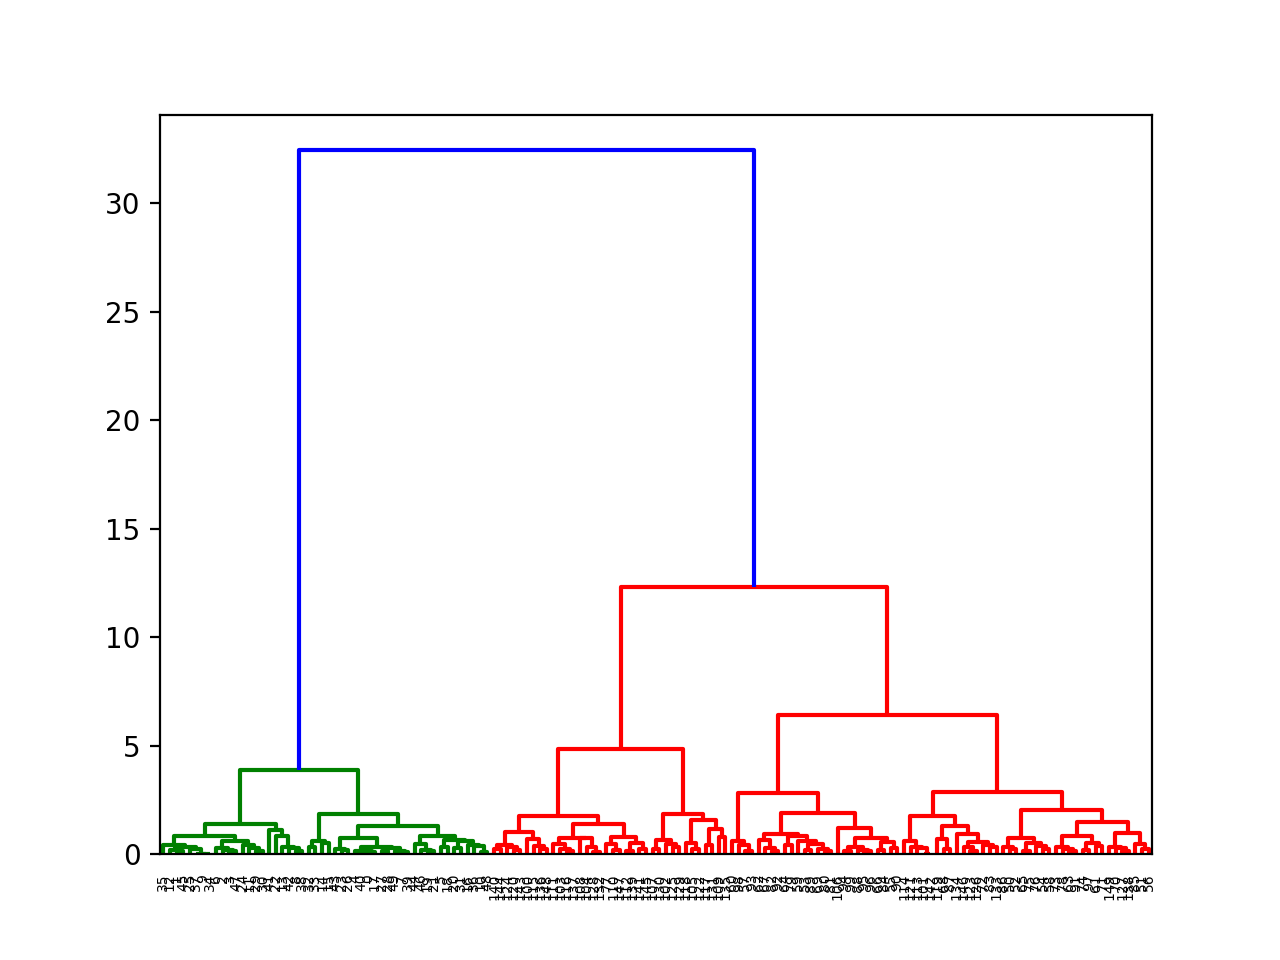
\includegraphics[width=1.0\textwidth]{./image/Figure_1}
    \caption{The Clustering plot}
    \label{}
\end{figure}
\begin{figure}[]
    \centering
    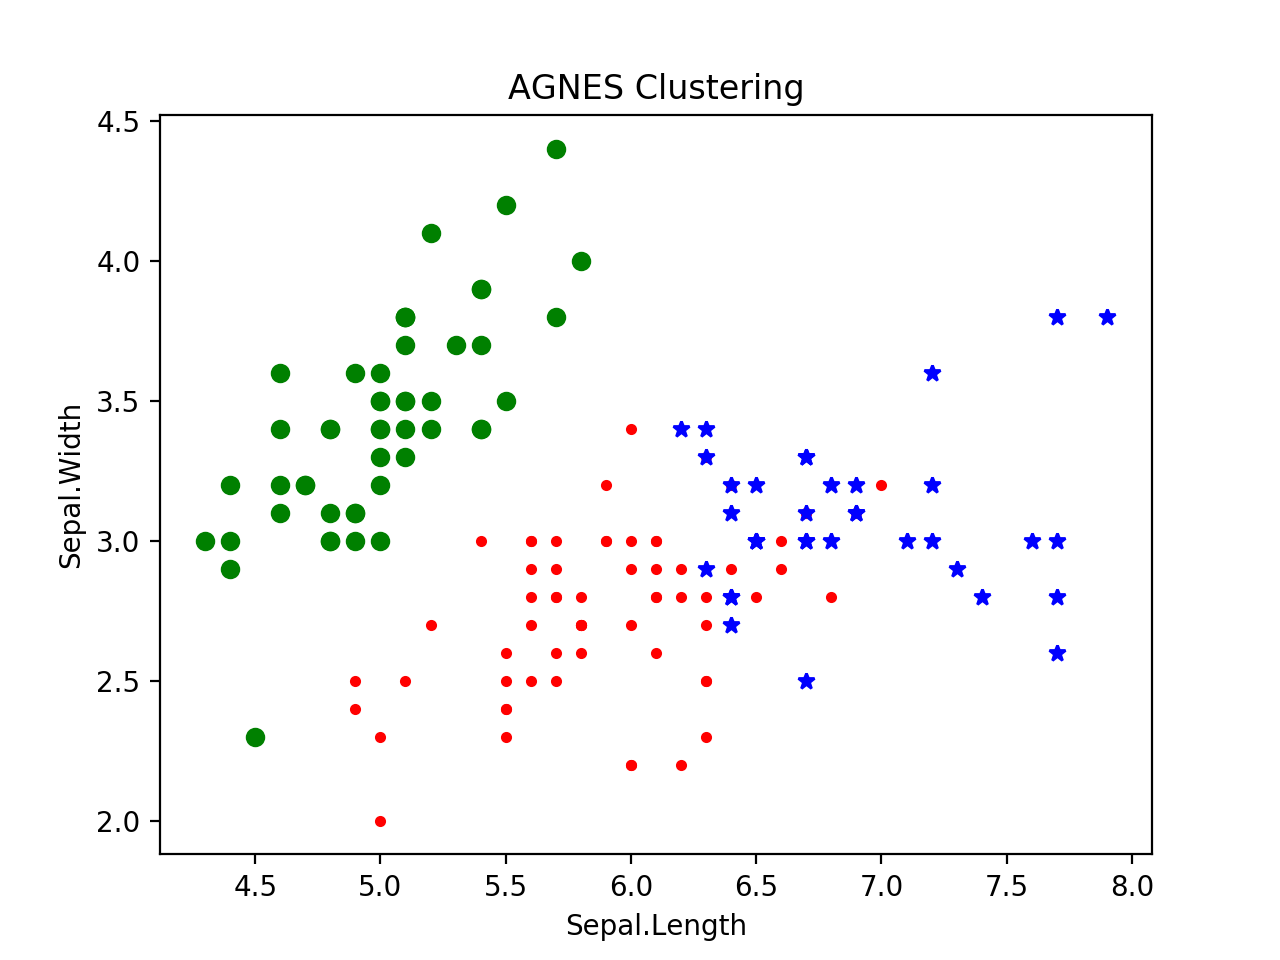
\includegraphics[width=1.0\textwidth]{./image/Figure_2}
    \caption{The Clustering graph}
    \label{}
\end{figure}
\end{homeworkProblem}
\end{document}
